\documentclass{standalone}

\usepackage[OT1]{fontenc}
\renewcommand*\familydefault{\sfdefault}
\usepackage{helvet,sfmath}
\usepackage{siunitx}

\usepackage{tikz}
\usetikzlibrary{arrows,calc,patterns}
% \usetikzlibrary{intersections, calc, arrows.meta}
\usepackage{tikz,tkz-euclide}

% \definecolor{square}{RGB}{177,162,202}

\begin{document}

\begin{tikzpicture}[scale=0.3]
    %% Background
    \draw[draw=none] (-30,-20) to (-30,10) to (30,10) to (30,-20) to (-30,-20);
    %% Figures
    \draw (-22.5,8) node[below]{ 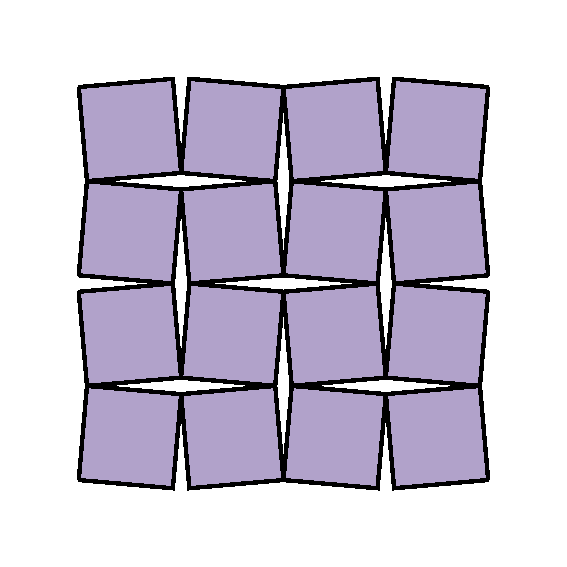
\includegraphics[width=3cm]{Problem_1/Figs_P1/10_Rotating_squares.pdf} };
    \draw (-7.5,8) node[below]{ 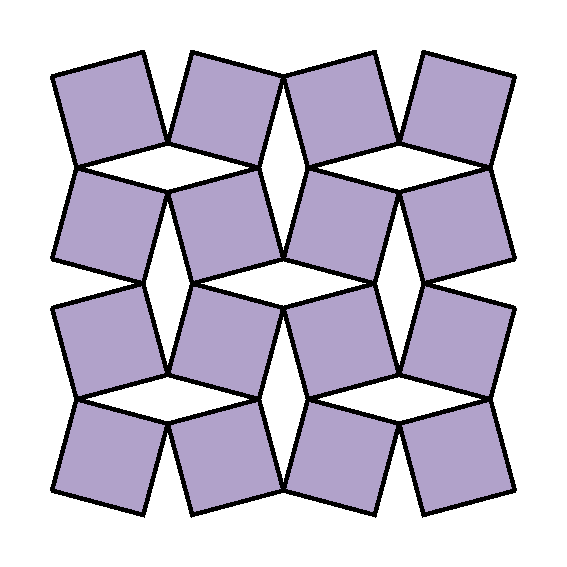
\includegraphics[width=3cm]{Problem_1/Figs_P1/30_Rotating_squares.pdf} };
    \draw (7.5,8) node[below]{ 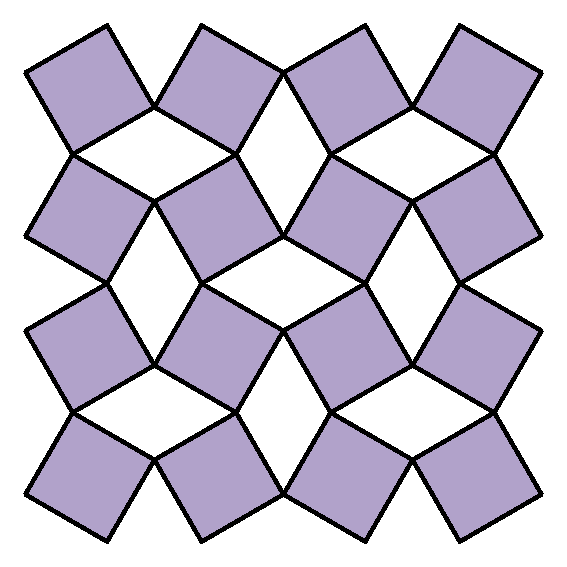
\includegraphics[width=3cm]{Problem_1/Figs_P1/60_Rotating_squares.pdf} };
    \draw (22.5,8) node[below]{ 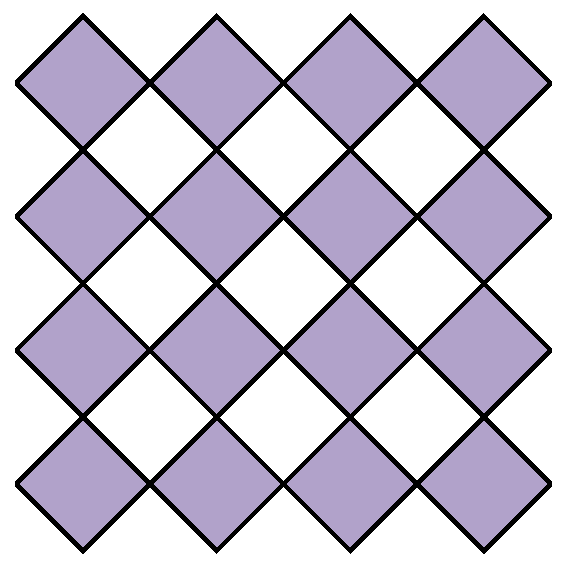
\includegraphics[width=3cm]{Problem_1/Figs_P1/90_Rotating_squares.pdf} };
    \draw (-22.5,-7) node[below]{ 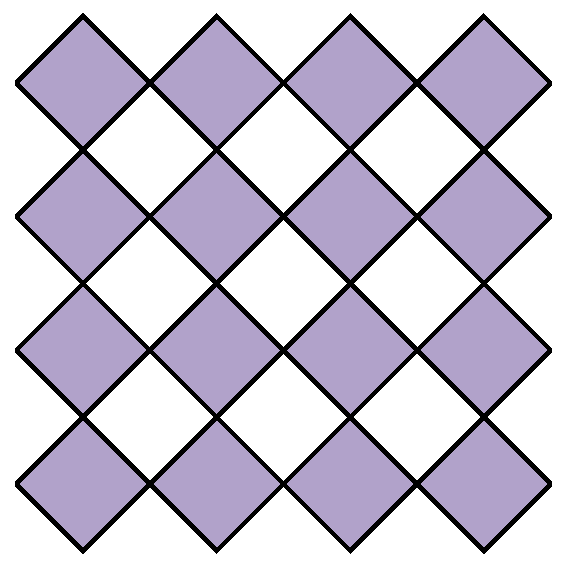
\includegraphics[width=3cm]{Problem_1/Figs_P1/90_Rotating_squares.pdf} };
    \draw (-7.5,-7) node[below]{ 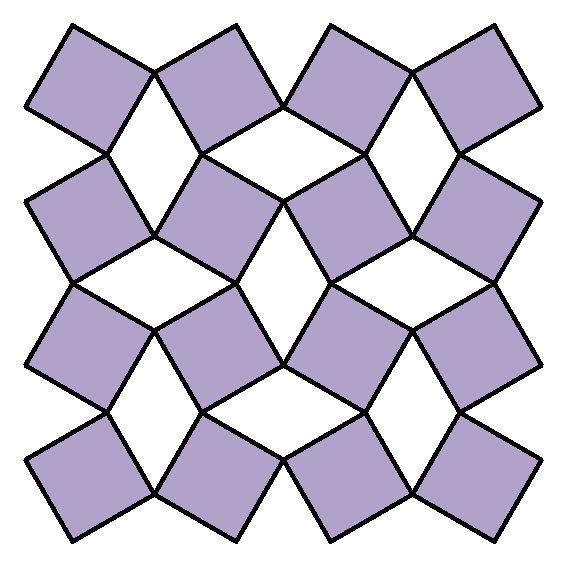
\includegraphics[width=3cm]{Problem_1/Figs_P1/120_Rotating_squares.pdf} };
    \draw (7.5,-7) node[below]{ 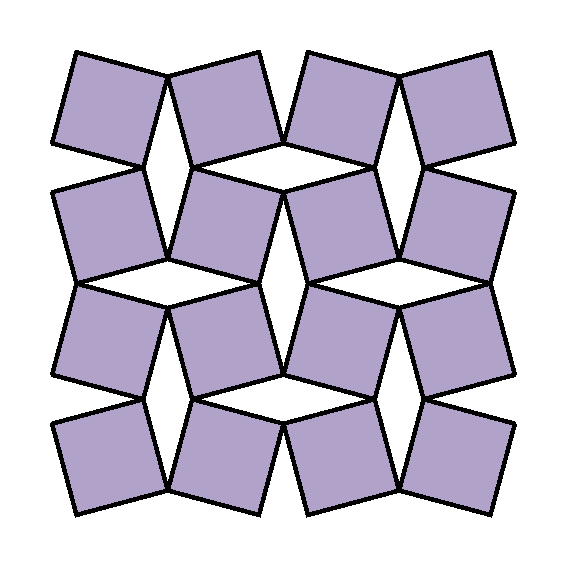
\includegraphics[width=3cm]{Problem_1/Figs_P1/150_Rotating_squares.pdf} };
    \draw (22.5,-7) node[below]{ 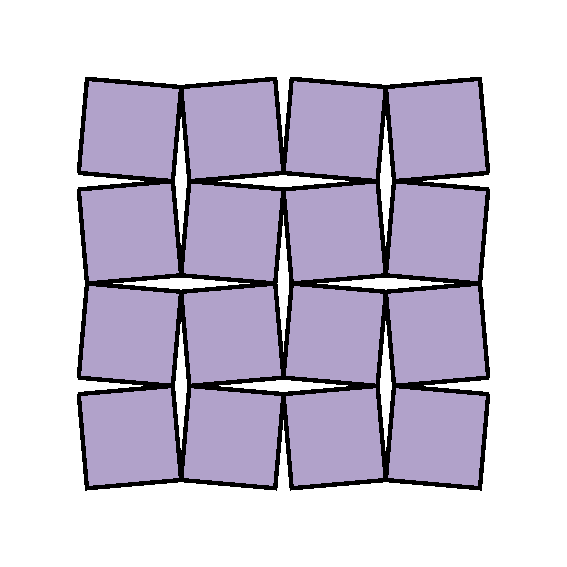
\includegraphics[width=3cm]{Problem_1/Figs_P1/170_Rotating_squares.pdf} };
    %% Notes
    \draw
    (-22.5,8.5) node{\(\theta=\SI{10}{^\circ}\)}
    (-7.5,8.5) node{\(\theta=\SI{30}{^\circ}\)}
    (7.5,8.5) node{\(\theta=\SI{60}{^\circ}\)}
    (22.5,8.5) node{\(\theta=\SI{90}{^\circ}\)}
    (-22.5,-6.5) node{\(\theta=\SI{90}{^\circ}\)}
    (-7.5,-6.5) node{\(\theta=\SI{120}{^\circ}\)}
    (7.5,-6.5) node{\(\theta=\SI{150}{^\circ}\)}
    (22.5,-6.5) node{\(\theta=\SI{170}{^\circ}\)}
    ;
    %% Arrows
    \draw[-Stealth, very thick] (-17,2.8) to (-13,2.8);
    \draw[-Stealth, very thick] (-2,2.8) to (2,2.8);
    \draw[-Stealth, very thick] (13,2.8) to (17,2.8);
    \draw[-Stealth, very thick] (-17,-12.2) to (-13,-12.2);
    \draw[-Stealth, very thick] (-2,-12.2) to (2,-12.2);
    \draw[-Stealth, very thick] (13,-12.2) to (17,-12.2);
\end{tikzpicture}

\end{document}
